%!TEX root = ../thesis.tex
%*******************************************************************************
%****************************** Second Chapter *********************************
%*******************************************************************************

\chapter{Theory}  %Title of the Second Chapter
\pagebreak

\ifpdf{}
    \graphicspath{{Chapter2/Figs/Raster/}{Chapter2/Figs/PDF/}{Chapter2/Figs/}}
\else
    \graphicspath{{Chapter2/Figs/Vector/}{Chapter2/Figs/}}
\fi


%********************************** % First Section  **************************************
\section{Rubidium} %Section - 1.1

\begin{figure}[h]
\centering
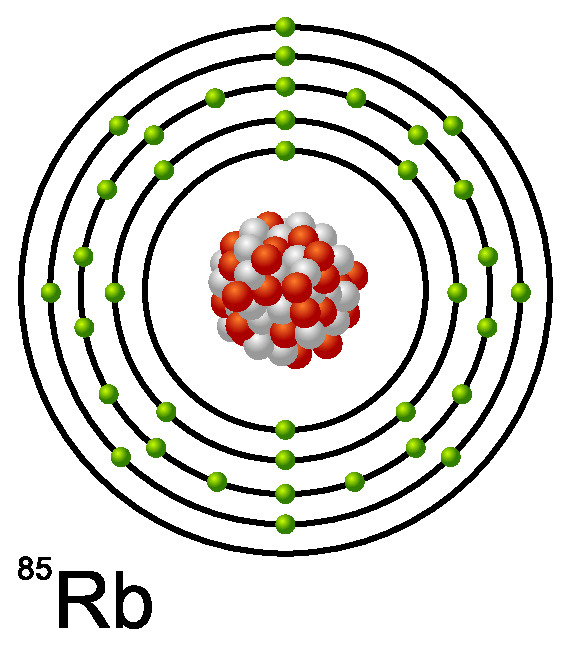
\includegraphics[width=0.3\textwidth]{rubidium_atom}
\caption[Rubidium Atom]{Schematical representation of \(^{85}\)Rb}
\label{fig:Atom}
\end{figure}

\vspace{\fill}

Rubidium is a chemical element with symbol Rb and atomic number 37.
It is a soft, silvery-white metallic element of the alkali metal group, 
with an atomic mass of 85.4678. Elemental rubidium is highly reactive, with 
properties similar to those of other alkali metals.\\


German chemists Robert Bunsen and Gustav Kirchhoff discovered rubidium in 
1861 by the newly developed technique, flame spectroscopy.
Because of the bright red lines in its emission spectrum, they chose a name 
derived from the Latin word rubidus, meaning ``deep red''. \citep{bunsen}\\

Although rubidium is monoisotopic, rubidium in the Earth's crust is composed of 
two isotopes: the stable \(^{85}\)Rb and the radioactive \(^{87}\)Rb. \citep{nubase}

\vspace{\fill}

\begin{table}[h]
\centering
\begin{tabular*}{0.5\textwidth}{@{\extracolsep{\fill} }l c c}
\toprule
& \multicolumn{2}{c}{Rubidium} \\
\midrule
Isotope & 85 & 87 \\
Atomic mass & 84.911794 & 86.909187 \\
in \(10^{-25}\)kg & 1.40999 & 1.44316 \\
Abundance & 72.17\% & 27.83\% \\
Spin I & \(\sfrac{5}{2}\) & \(\sfrac{3}{2}\) \\
\bottomrule
\end{tabular*}
\caption{Properties of rubidium isotopes}
\label{table:iso_prop}
\end{table}
\pagebreak

%********************************** % Second Section  **************************************
\section{D2 line} %Section - 1.2 

\begin{figure}[h]
\centering
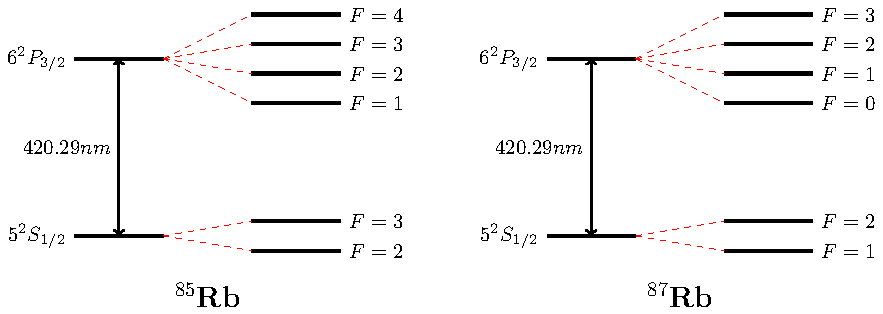
\includegraphics[width=0.9\textwidth]{energylevel}
\caption{\(5^{2}S_{1/2} \rightarrow 6^{2}P_{3/2}\) transition of \(^{85}\)Rb and \(^{87}\)Rb with corresponding hyperfine structure}    
\end{figure}

\vspace{\fill}

As we can see both isotopes have the same transition energy, but due to the different spin I (see table:~\ref{table:iso_prop}) we get
different energy levels for the groundstate \citep{nist_asd}. This is the reason why we wittness four doppler peaks in our spectrum. \\

\textbf{Caution:} Both figures below show the correct correlation between energy and isotopes. The explanation of this is that higher
energy levels need lesser transition energy to reach the same excited state. 

\vspace{\fill}

\begin{figure}[h]
\centering
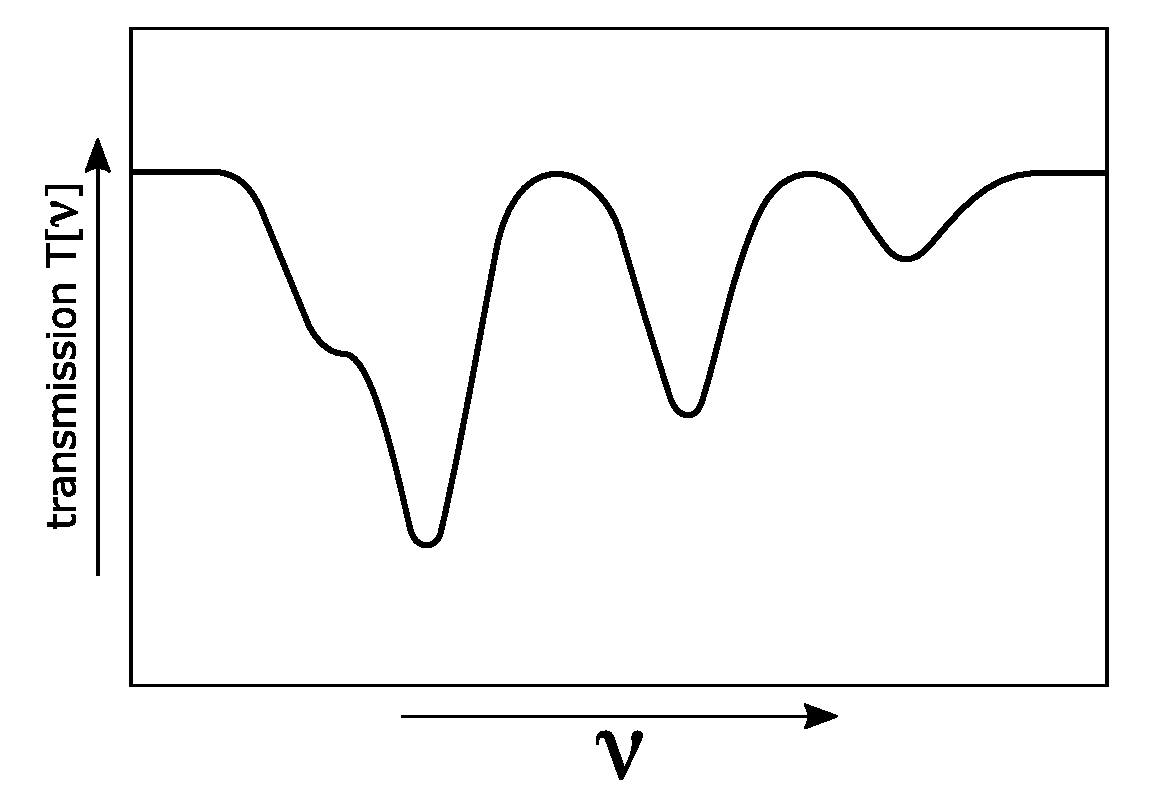
\includegraphics[width=0.6\textwidth]{spectrum_doppler}
\caption{Doppler spectrum of D2 line}
\label{fig:doppler} 
\end{figure}

\vspace{\fill}
\pagebreak

\begin{figure}[h]
\centering
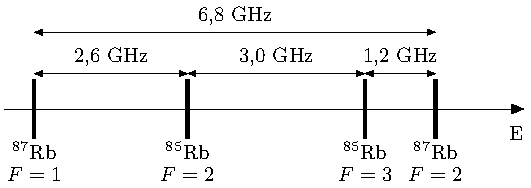
\includegraphics[width=0.6\textwidth]{groundstate}
\caption{Relative energy gaps of the groundstates between both isotopes}
\label{fig:gap} 
\end{figure}

%********************************** % Third Section  *************************************
\section{Two-level atom} %Section - 1.3

In the upcomming sections we will derive an expression for the absorbtion or to be precise the
intensity of the laser beam, but first we have to discuss the model on which basis we will do this.\\

The simplest model is the two-level atom with a groundstate \ket{g} and one excited state \ket{e}. There are three
possible transitions:\\

\begin{minipage}[c][][c]{.35\textwidth}
\begin{itemize}
\item[(1)] absorbtion
\item[(2)] stimulated emission
\item[(3)] spontaneous emission
\end{itemize}
\end{minipage}
\hfill
\begin{minipage}[c]{.55\textwidth}
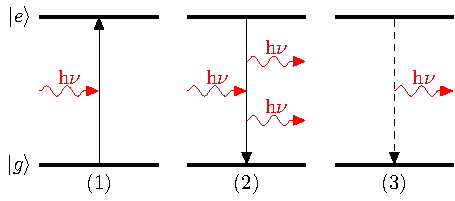
\includegraphics[width=\textwidth]{twolevel}
\captionof{figure}{Two-level atom model}
\end{minipage} \\ \\


In our case we will only consider the photon absorbtion. 

\pagebreak
%********************************** % Fourth Section  *************************************
\section{Laser absorbtion}  %Section - 1.4

\pagebreak
%********************************** % Fifth Section  *************************************
\section{Doppler shifts}  %Section - 1.5

\pagebreak
%********************************** % Sixth Section  *************************************
\section{Behavior of absorbtion coefficient}  %Section - 1.6

\pagebreak
%********************************** % Seventh Section  *************************************
\section{Non-linear differential equation}  %Section - 1.7

\pagebreak